\subsection{System Monitor}

\subsubsection{Objective and Functionality}
The System Monitor is a pivotal component in a biometric data-based framework for user access and verification. It serves one main function: Showing the user data in a screen. The System Monitor's functionalities include:
\begin{itemize}
    \item Subscribing to and processing location data from two ESP-01 modules with ultrasonic sensors via MQTT.
    \item Subscribing and processing user data from the user data collector system and showing it via the screen
    \item Subscribing and showing the user identity into the screen.
    \item Visually representing user proximity using an LED bar.
\end{itemize}

\subsubsection{Project Definition and Milestones}
The development of the System Monitor involved the following milestones:
\begin{enumerate}
    \item Establishing MQTT communication.
    \item Integrating and configuring the LED bar and LCD with the ESP32
    \item Developing and testing the software for and data display.
    \item Efficient multitasking and task synchronization within FreeRTOS.
\end{enumerate}

\subsubsection{Achieved milestones, execution order, priority, and dependencies}
\begin{enumerate}
    \item \textbf{Milestone 1: Establishing MQTT Communication}
        \begin{itemize}
            \item \textit{Priority:} High. Fundamental for data transmission.
            \item \textit{Dependencies:} Basic WiFi setup.
            \item \textit{Execution Order:} First, as it is crucial for data reception.
            \item \textit{Assigned to:} Ferran
        \end{itemize}

    \item \textbf{Milestone 2: LED Bar and LCD Integration}
        \begin{itemize}
            \item \textit{Priority:} Medium. Important for user interface.
            \item \textit{Dependencies:} Successful MQTT setup.
            \item \textit{Execution Order:} Second, building upon established communication.
            \item \textit{Assigned to:} Alex, Pablo
        \end{itemize}

    \item \textbf{Milestone 3: Software Development}
        \begin{itemize}
            \item \textit{Priority:} High. Essential for functionality.
            \item \textit{Dependencies:} Functional hardware setup.
            \item \textit{Execution Order:} Third, focusing on processing and display.
            \item \textit{Assigned to:} Pablo
        \end{itemize}

    \item \textbf{Milestone 4: Multitasking and Task Synchronization}
        \begin{itemize}
            \item \textit{Priority:} High. Critical for system reliability.
            \item \textit{Dependencies:} Completion of initial software development.
            \item \textit{Execution Order:} Fourth, finalizing the system integration.
            \item \textit{Assigned to:} Pablo
        \end{itemize}
\end{enumerate}

\subsubsection{Hardware Development}
The hardware setup for the System Monitor comprises:
\begin{itemize}
    \item An ESP32 microcontroller connected to a breadboard.
    \item An LED bar and an LCD screen interfaced with the ESP32 for display.
\end{itemize}

\subsubsection{Interaction with Other Components}
The System Monitor interacts with the ESP-01 modules to determine the user's location based on distance data, the user data collector system, and the rpi user authentication system.  Everything is then displayed on the LED bar and LCD screen.

\subsubsection{Dedication Time}
Approximately 30 hours were dedicated to developing the System Monitor, focusing on both hardware assembly and software programming.

\subsubsection{User Story}
As a user approaches, the System Monitor detects their presence, lighting up the LED bar and displaying their approximate location (left, right, or center) on the LCD screen, providing real-time feedback.
When the user uses the data collector system, the user shows the current heart rate and galvanic data, and when the raspberry authenticates the user (using the data and a camera) it shows it's name on the screen

\subsubsection{Challenges and Solutions}
\begin{itemize}
    \item \textbf{Hardware Challenges:} Complex wiring and space constraints on the breadboard, along with troubleshooting LED issues.
    \item \textbf{Software Challenges:}
        \begin{enumerate}
            \item Establishing reliable communication and processing the proximity data accurately (when it's center? when it's on the right? etc)
            \item The synchronization system using rtos was a pain. Altough the documentation was good, the ESP-32 didn't do allways the same things running the same code (and we're using mutex locks....).
        \end{enumerate}
\end{itemize}

\subsubsection{Hardware and Software Integration}
\begin{figure}[ht]
    \centering
    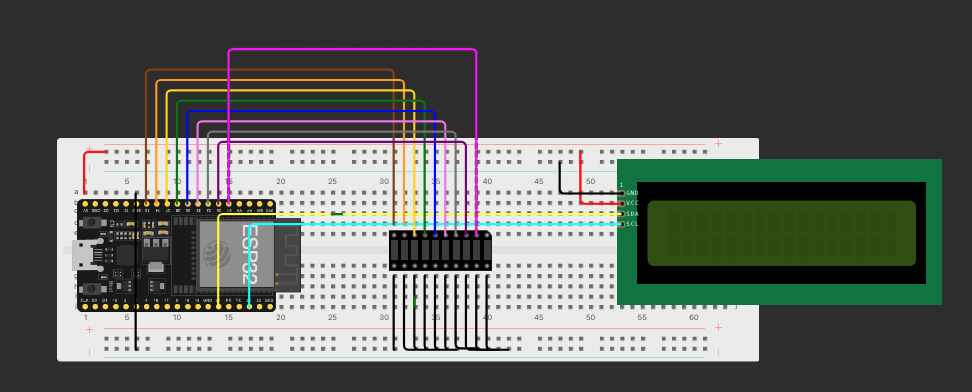
\includegraphics[width=0.8\textwidth]{../images/activity_monitor_scheme.png}
    \caption{ESP32 with LED bar and LCD display connected on a breadboard.}
    \label{fig:esp32_system_monitor}
\end{figure}

\subsubsection{Microcontroller Interaction Protocol}
The System Monitor project involves coordinated communication between multiple microcontrollers, primarily the ESP32, the two ESP-01 modules, the Arduino 33 BLE, and the raspberry pi 4. The communication is structured as follows:

\paragraph{Communication Protocol}
The project utilizes the MQTT (Message Queuing Telemetry Transport) protocol, a lightweight and efficient messaging protocol ideal for IoT applications. This protocol is chosen for its low bandwidth usage and its ability to provide reliable communication over WiFi.

\subsubsection{MQTT Tree Structure}
The MQTT protocol in the System Monitor project uses a structured approach to manage the data flow. Below is the outline of the MQTT topics and their functions:

\paragraph{MQTT Topics}
The ESP-32 subscribes to the following topics for retreiving all the data:
\begin{itemize}
    \item \textbf{sensor1/distance:} This topic is used by the first ESP-01 module. It publishes the distance data measured by its connected ultrasonic sensor. The ESP32 subscribes to this topic to receive updates on the user's distance from this sensor.
    \item \textbf{sensor2/distance:} Similar to the first, this topic is for the second ESP-01 module. It provides distance data from its sensor, allowing the ESP32 to determine the user's location relative to this second sensor.
    \item \textbf{rpi/prediction:} Topic that shows the name of the user identified.
    \item \textbf{sensor3/heart}: Gets the heart rpm.
    \item \textbf{sensor3/galvanic}: Gets the galvanic data
\end{itemize}
